At the beginning of the 20$\textsuperscript{th}$ century the world underwent the first quantum revolution. New ideas about wave-particles duality and quantization gave scientists the tools to explain previously observed phenomena such as the periodic table. With a deeper understanding, this new quantum theory drove revolutionary technologies such as electronic semiconductors thus bringing the world into the Information age. Now we are undergoing a second quantum revolution where we are no longer using quantum mechanics to simply explain observed phenomena, we are actively \textit{controlling} quantum mechanics.\cite{Dowling2003} We are using quantum technologies to organize and build complex systems at the atomic level. This extraordinary leap forward has allowed us to create and research new quantum phases of matter and their associated new quasi-particles. Aside from the importance of understanding novel fundamental physics, research into new quantum phases of matter is paramount for driving new technologies forward. For example, research into high-temperature superconductivity may lead us to room-temperature superconductivity, a phenomena which would massively reduce energy dissipation in modern electronics. In this dissertation, we describe the development of new equipment to help build these new quantum tools as well as the novel iron-based topological superconducting system such equipment has allowed us to probe.
\section{Scope}
The works presented in this dissertation fall into two main parts: advances in nano-fabrication equipment and topological superconductivity. The first part introduces recent advances in condensed matter physics along with the difficulties associated with fabricating electronic devices to better study these new topics. In particular, we discuss materials that are acutely air-sensitive such as GdTe$_{3}$ as well as materials that are stable in air but have air-sensitive surfaces such as \ac{FTS}. The second part dives into the subject topological superconductors and higher order topology. Specifically, we focus on the iron-based superconductor \acl{FTS}, its topological properties, and some exciting new experiments.\par
The rest of this introduction will review pertinent background material. We introduce the notion of emergence and quantum phases of matter with specific applications to superconducting materials. We will leave some of the more advanced subjects of superconductivity, e.g. tunneling into a superconductor from a normal metal, to the appendices where these subjects can get a more in-depth treatment. A brief overview of topology will be given but more focus will be spent on how to treat the notion of topology in superconductivity.
\section{Emergence and New Phases of Matter}
Emergence can be colloquially summarized as, ``The whole is greater than the sum of its parts." Examples of emergence are all around us from the biggest of scales where galaxies coalesce into superclusters to the smallest of scales where atoms emerge out of the fundamental excitations of quantum fields. With such a huge subject it may be difficult to see how this concept is useful in driving a research direction. Thus to keep this work on track we will use the sharper definition provided by Kivelson \& Kivelson:
\begin{quote}
	``An emergent behavior of a physical system is a qualitative property that can only occur in the limit that the number of microscopic constituents tends to infinity."\cite{Kivelson2016}
\end{quote}
Using this definition, it is evident that emergence heavily influences condensed matter systems. Indeed, phases of matter are a prime example of emergence as a single crystal can exhibit wildly different properties depending on \textit{external} conditions.
\par 
Many of these phases of matter can be described elegantly through the language of symmetry and symmetry breaking\cite{Noether1918, Landau1937, pathria_beale_2022}. Quantum Hall Effect. Symmetry cannot explain everything. Topology! Berry Phase! Using symmetry and topology together we can fabricate awesome new phases with new quasiparticles. Example above the new quasiparticle is the 1D dispersionless edge mode. 
\section{Topological Superconductivity}
Smooth transition from general topology to topological superconductivity in particular. Topological superconductivity 
An in-depth derivation of the \ac{BdG} equations for superconductivity are presented in Appendix \ref{app:ARfit}, here we will use the final Hamiltonian from that appendix with some minor alterations. We will be closely following the works of Kitaev and Bernevig \& Hughes\cite{Kitaev2001, bernevig_hughes_2013}.\par 
We begin by describing a 1-D chain of fermions, i.e., at each lattice site $j$ on the chain there is a complex fermion $c_{j}$. For simplicity, we consider these complex fermions to either be spinless or fully spin-polarized due to a source of time-reversal symmetry breaking. Since a momentum-independent s-wave pairing potential is not possible for spinless fermions, we will use a momentum-dependent p-wave potential (in momentum space):
\begin{align}
	H_{\Delta} = \frac{1}{2}\left(\Delta pc_{p}^{\dagger}c_{-p}^{\dagger}+\Delta^{*}pc_{-p}c_{p}\right)
\end{align}
where $c^{\dagger}$ and $c$ are the creation and annihilation operators, $p$ is the momentum, and $\Delta$ is the superconducting pairing potential. The lattice \ac{BdG} Hamiltonian (in real space) we need to solve is:
\begin{align}
	H_{BdG} = \sum_{j}\left[-t\left(c_{j}^{\dagger}c_{j+1}+c_{j+1}^{\dagger}c_{j}\right)-\mu c_{j}^{\dagger}c_{j}+|\Delta|\left(c_{j+1}^{\dagger}c_{j}^{\dagger}+c_{j}c_{j+1}\right)\right]
\end{align}
where $t>0$ is the hopping parameter and $\mu$ is the chemical potential. To investigate how each parameter affects the superconducting gap, we take a lattice Fourier transform to convert back into momentum space:
\begin{align}
	H_{BdG} = \frac{1}{2}\sum_{p}\Psi_{p}^{\dagger}
	\begin{pmatrix}
		-2t\cos(p)-\mu & 2i|\Delta|\sin(p)\\
		-2i|\Delta|\sin(p) & 2t\cos(p)+\mu
	\end{pmatrix}
	\Psi_{p}
\end{align}
where $\Psi_{p}=(c_{p}\quad c_{-p^{\dagger}})$. Diagonalizing the Hamiltonian gives the energy eigenvalues as:
\begin{align}
	E_{\pm}(p) = \pm\sqrt{(2t\cos(p)+\mu)^{2}+4|\Delta|^{2}\sin^{2}(p)}
\end{align}
These eigenbands are plotted in Fig \ref{pwavesc} for various values of $\mu$ and setting $t$ and $|\Delta|$ both to 1. From these bands we can see the gap closes when $\mu=-2t$ with energy gaps for both $\mu>-2t$ and $\mu<-2t$. As it turns out, the energy gaps for $\mu < -2t$ are topologically non-trivial while the energy gaps for $\mu > -2t$ are trivial.
\begin{figure}
	\centering
	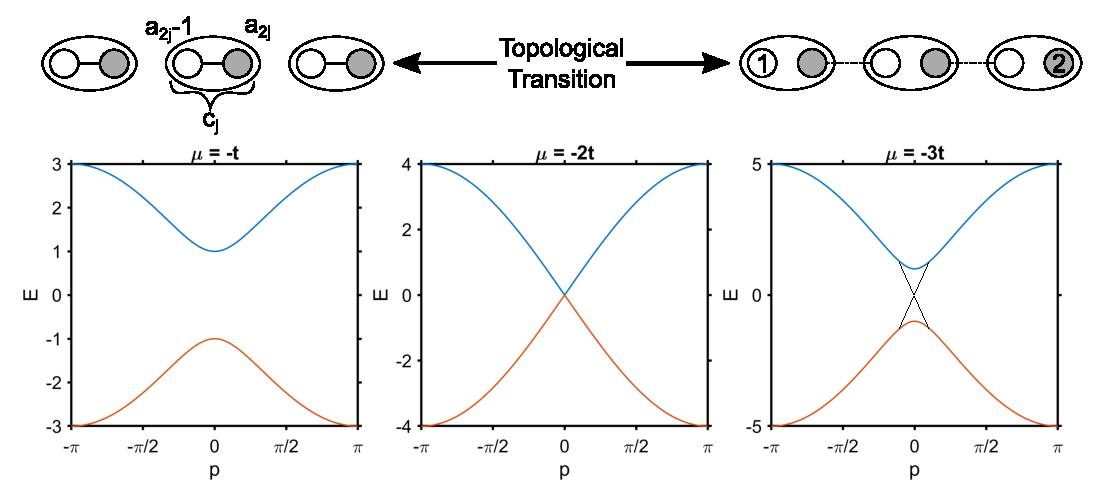
\includegraphics[width=\textwidth]{Intro/Figures/PWave_SC.eps}
	\caption{Dispersion relations of a 1D p-wave superconductor plotted at three different $\mu$ values. a) The trivial p-wave pairing scenario. The individual majorana particles each couple to the majorana on the same site. b) The critical value for $\mu$ where the gap closes. c) The topological p-wave pairing scenario. The majorana particles pair with majoranas on the nearest-neighbor site instead of on the same site. Two majorana zero modes are left on the edges of the wire, consistent with the bulk-boundary correspondence.}
	\label{pwavesc}
\end{figure}
For an intuitive picture for why this is we will split the complex fermion operators into their Majorana fermion constituents. We replace each complex fermion $c_{j}$ with two Majorana fermions, $a_{2j-1},a_{2j}$ via $c_{j}=\frac{1}{2}(a_{2j-1}+ia_{2j})$ and $c_{j}^{\dagger}=\frac{1}{2}(a_{2j-1}-ia_{2j})$. The Majorana operators are fermionic and are defined by their property $a_{j}=a_{j}^{\dagger}$ therefore they satisfy $\{a_{j}^{\dagger},a_{j'}\}=2\delta_{jj'}$ as well as $\{a_{j},a_{j'}\}=2\delta_{jj'}$. As an aside, due to the latter relation we can always break up a complex fermion operator into its real and imaginary Majorana components, although it may not always be a useful representation. Now, the Hamiltonian for the lattice p-wave superconductor can be written as:
\begin{align}
	H_{BdG} = \frac{i}{2}\sum_{p}\left(-\mu a_{2j-1}a_{2j}+(t+|\Delta|)a_{2j}a_{2j+1}+(-t+|\Delta|)a_{2j-1}a_{2j+2}\right)
\end{align}
Here we can examine the difference between the two cases presented above by looking at two special limits.\par 
The first limit is the trivial phase when we choose $\mu < 0$ and $|\Delta|=t=0$. Here, the Hamiltonian reduces to,
\begin{align}
	H = -\mu\frac{i}{2}\sum_{j}(a_{2j-1}a_{2j})
\end{align}
In this phase, the Majorana operators on each site are coupled together with an energy $\mu/2$ but there is no coupling between Majorana operators on different sites (see Fig \ref{pwavesc}). This is denoted as the trivial phase since there will be no low-energy states on the end of the chain if the boundaries are cut between sites. Said another way, the Majorana operators are localized to each site and are therefore in the atomic limit which is to say the trivial ground state.\par 
The second limit is the topological phase where we choose $|\Delta|=t>0$ and $\mu=0$. Here, the Hamiltonian reduces to,
\begin{align}
	H=it\sum_{j}a_{2j}a_{2j+1}
\end{align}
This phase is the opposite of the previous phase as the Majorana operators on each site are only coupled to Majorana operators on \textit{different} sites with an energy $t$. When the chain is cut the Majorana operators $a_{1}$ and $a_{2L}$ ($L$ is the last site) are ``unpaired" and therefore there is a low-energy state on the each end of the chain (see Fig \ref{pwavesc}). Comparing to before, it is impossible to adiabatically tune this phase back to the atomic limit and is thus a topologically non-trivial state.\par 
